\documentclass[12pt]{article}
\usepackage{amsmath,amssymb,amsthm}
\usepackage{graphicx,mathabx}
\usepackage{xcolor}
\usepackage{tikz}
\usepackage{placeins}
\usepackage{lipsum}
\usepackage[shortlabels]{enumitem}
\usepackage{placeins}
\usepackage[makeroom]{cancel}
\newcommand\tab[1][1cm]{\hspace*{#1}}
\begin{document}
\title{TCSS 343 - Week 4}
\author{Jake McKenzie}
\maketitle
\noindent\centerline{\textbf{Dynamic Programming}}\\\\\\\\\\\\\\\\
\begin{center}
    ``An optimal policy has the property that whatever the initial state and initial decision are, the remaining decisions must constitute an optimal policy with regard to the state resulting from the first decision." \\$\cdots$\\  Richard Bellman's \textbf{Principle of Optimality}
\end{center}
\begin{center}
    ``What we choose means more than what was handed to us by chance." \\$\cdots$\\  Ada Palmer
\end{center}
\begin{center}
    `` If `dynamic programming' didn't have such a cool name, it would be known as 'populating a table'". \\$\cdots$\\ Mark Dominus 
\end{center}
\newpage
\noindent 1. Today we're going to explore dynamic programming. Below are three implementations of the fibonacci algorithm that I wrote in python. I want you to draw the \textbf{``tree"} for each then reflect on how the ``bottom up" apprach is different from the other two? (Hint: They are all trees but also different types of trees. This is a key insight in my opinion in idea in understanding dynamic programming) \\
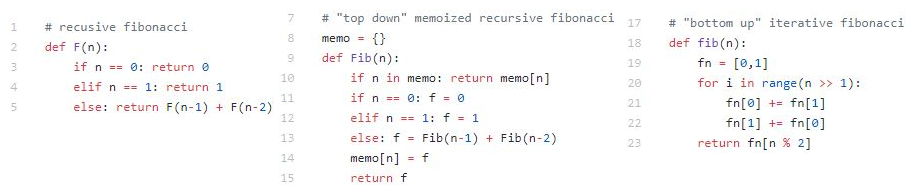
\includegraphics[width=\linewidth]{fib.jpg}
\newpage

\noindent 2. I found these really cool recursive Fibonacci formulas: 
$F_{2n+1}=F_{n+1}^{2}+F_{n}^{2}$ and $F_{2n}=2F_{n+1}F_{n}-F_{n}^2$
 now can you use them to find $F_{11}$ and $F_{10}$(worth noting that
 $F_2 = 1$, $F_1 = 1$, and $F_0 = 0$)?\\\\\\\\\\\\\\\\\\\\
 3. Can you now write an iterative method that computes $F_{2n}$ and $F_{2n+1}$
 using dynamic programming?\\\\\\\\\\\\\\\\\\\\\\\\\\\\\\\\\\\\\\\\
 4. How is this different from the basic Fibonacci formula? What is the
 time complexity of this function? Space complexity?
    \FloatBarrier
\newpage
\centerline{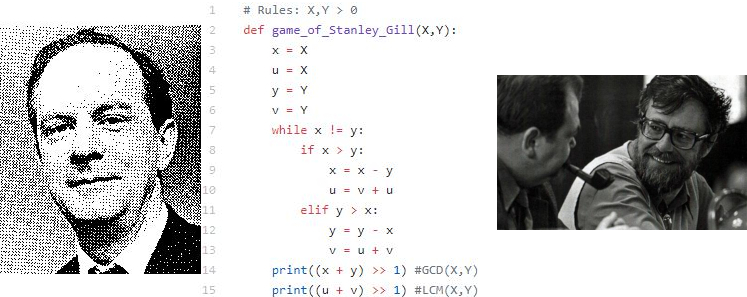
\includegraphics[scale = 2]{comb.jpg}}
\noindent 5. This is a game shown to Edsgar Dijkstra(pictured right) when he was still an undergraduate, attributed to Stanley Gill(pictured left), an early computer scientist. Now it is true that $2XY = xv+yu$, which can be seen when the variables are initialized. But it is always true given that $X,Y > 0$? Show why this is true. (Hint: You can use the comments to help you along. Remember that the $>> 1 $ operation is the same as $ / 2$.)
\newpage
\noindent 6. Hopefully in problem 1 I was able to impart on you the reality that most dynamic 
programming problems can be thought of as graph problems, specifically directed acyclic graphs, 
DAG for short. Even if you don't solve them with DAGs I think it's a useful headspace for a large class of problems. 
We can typically solve DP problems without constructing a graph. If we aren't going to use a graph there are other useful
tools that you may not have run across. Let's try to understand what a bitmask is. I've been peppering
them into the packets all quarter but let's finally dive deep into them. Mask in bitmask means hiding 
something. Bitmask is nothing but a binary number that represents something.\\\\
Please connect the corresponding ``bitmask" with their
set operations or arithmetic operations. I encourage you to 
play around with the operation and really try understand what
they're doing. All operations are on two intergers $X$ and $Y$. 
I know this may seem disjointed from what you've covered in
class but I have used all of these in solving DP problems. 
Often times we aren't just worried about our time complexity,
but we're also worried about space complexity. Using integers
instead of arrays to represent data is sometimes vital in solving
hard problems. For example: we may represent the set $\{5,4,3,2,1\}$ 
as $11111$ in binary which is $31$ in decimal and the set $\{4,2,1\}$ 
as $01011$ in binary which is $11$ in decimal.
\begin{enumerate}[a)]
    \item  $X \& 1 \tab\tab\tab$ I)Union of two sets
    \item  $X \wedge Y \tab\tab\tab$ II)Arithmetic negation
    \item  $ (X >> 31) \& 1 \tab\tab$ III)Test for set membership
    \item  $X | Y \tab\tab\tab\tab$IV)2 to the power of X(also Singleton Set)
    \item  $X \& Y \tab\tab\tab\tab$V)Barrel shift left
    \item  $X \&= (X - 1) \tab\tab\tab$VI)Intersection of two sets
    \item  $(X<<Y) | (X >> (32 - Y))\tab$VII)Signed bit
    \item  $ ! X + 1 \tab\tab\tab\tab$IX)Clears lowest ``ON" bit in X
    \item  $1 << X \tab\tab\tab\tab$X)Symmetric Difference of two sets
    \item  $(X \& (1 << Y))$ $!= 0 \tab\tab$XI)Even/Odd check 
    \end{enumerate}
\newpage
\noindent 7. The N-Queens is one of the classic brain teasers. The problem can be stated simply:
On a NxN square checkerboard, place N queens in a way so that no queen threatens any 
of the other ones, ie. shares column, row or diagonal.\textbf{Below I will ask you a series of questions 
on how you might make a plan of attack to solving this problem.} Below are all possible ``unique" solutions
for an $N=8$. There are actually $92$ correct solutions in all. It's worth noting why we need dynamic
programming for such a problem. There are $\frac{64!}{(64-8)!8!}$ ways of arranging $8$ queens on a
chessboard.
\centerline{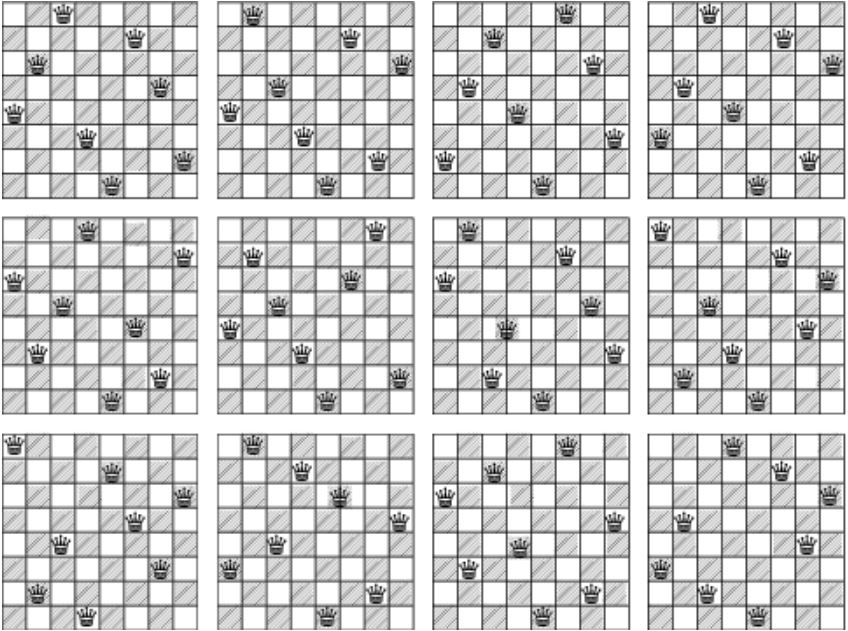
\includegraphics[scale = .25]{queen.jpg}}\\
7.0 How many (non-unique)solutions are there for $N = 1,2,3,4,5,6$\\\\\\\\
7.1 What are the subproblems to the global problem of computing all possible solutions to this problem?\\\\\\\\\\
7.2 What are the possible guesses to the solutions to this problem?\\\\\\\\\\
7.3 Using 5.1 and 5.2 can you come up with a recurrence that relates subproblem solutions?\\\\\\\\
7.4 Do your subproblems follow some order that is valid?
\newpage
\noindent 8. Do not attempt this page until you put a 
lot of thought and care into problem 5. Please write
some code that attempts to produce a solution to the
N-Queen problem.
 I understand that solving problems like this on the 
 fly can be difficult. I know when I was in seminar 
 I found it to be difficult. Writing code on paper sucks.
  Try your best, I believe in you. Please come up with your
  own solution. There are many, many ways to solve this,
  and I want your attempt, not the internets.
\newpage
\noindent 9. Time for some graph review. Shortest path algorithms on graphs all fixated 
on the concept of relaxation. To put simply, relaxing an edge from
one vertex to another means temporarily violating the shortest path
criteria locally to check to see if you can find a new global shortest path.
The relaxation algorithm is as follows(some python code for it):\\\\
\centerline{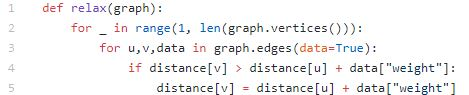
\includegraphics{relax.jpg}}\\
Why is the relaxation algorithm safe? Can you use the triangle inequality to
 prove it? Use this lemma: The relaxation algorithm maintains the 
 invariant that V.d$ \geq \delta$(S,V)$ \forall $v$ \in $V\\\\\\\\
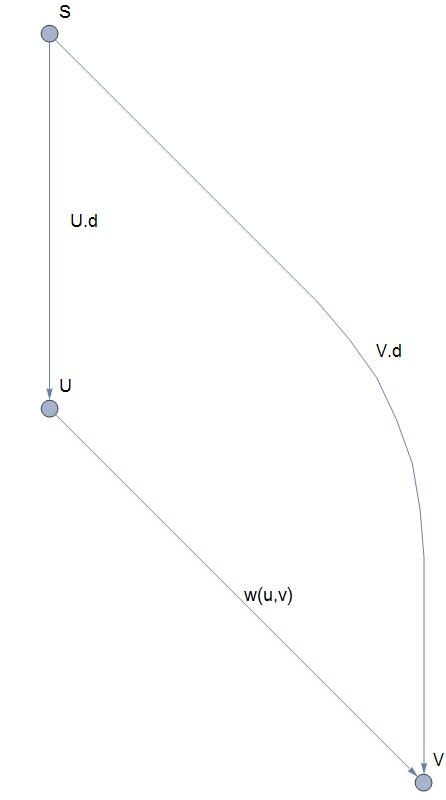
\includegraphics[scale = 0.35]{graph.jpg}\\
Triangle inequality: $\delta$(S,V) $\leq \delta$(S,U) $+ \delta$(U,V)
\newpage
\noindent A. Say you have access to a function \textbf{dict} that returns true 
if its input is a valid English word, and false otherwise. We are given 
as input a sentence from which the punctuation has been
stripped (for example: ``dynamicprogrammingisfabulous"). 
Assuming calls to dict take unit time, give an $O(n^2)$ time 
algorithm to figure out whether an input string of length n can be
split into a sequence of valid words or not. 
HINT: Try to remove valid words from the end of the input string.
\newpage
\noindent \centerline{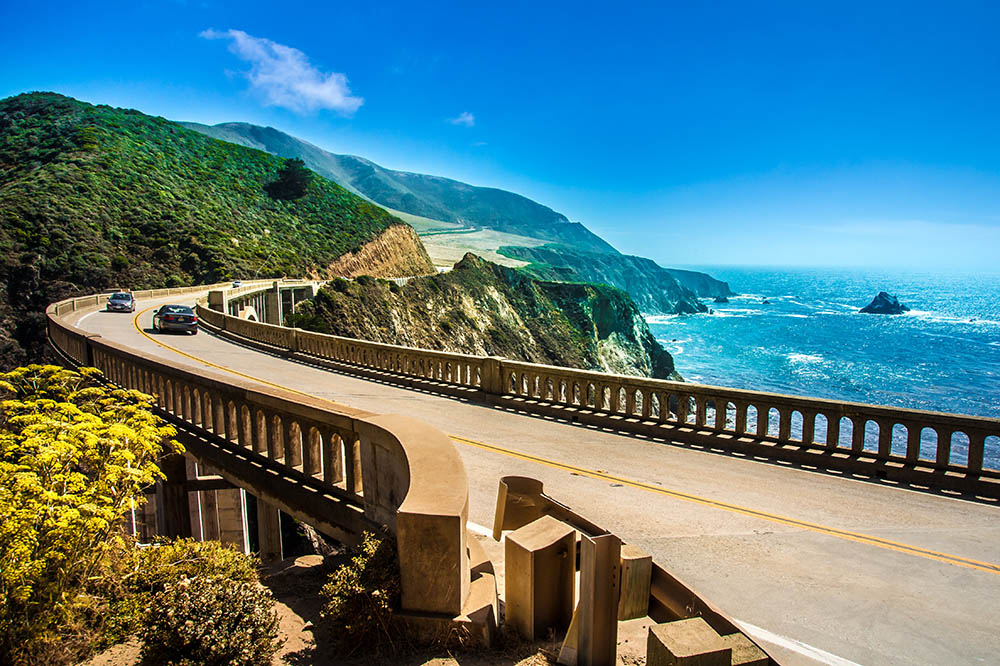
\includegraphics[scale = 1.25]{brix.jpg}}\\
B. So imagine you've graduated from University of Washington
in Tacoma and you got a nice job at a startup in San Francisco. It's the weekend
and you want to drive down to Monterrey to enjoy some wine with friends.
Now depending on what scenery you're driving through you find yourself
speeding through that locale for each time unit you're in it. It's the weekend
you don't really care how much time it takes you to get to Monterrey, but you
defintely don't want a ticket. What's the maximum amount of scenic value you can get
out of your weekend drive to Monterrey?

\begin{table}[]
    \begin{tabular}{|l|l|l|l|}
    \hline
    r & $sp_r$ & $sc_r$ \\ \hline
    1 & 5    & 1    \\ \hline
    2 & 9    & 6    \\ \hline
    3 & 26    & 18    \\ \hline
    4 & 31    & 22    \\ \hline
    5 & 36    & 28    \\ \hline
    \end{tabular}
    \end{table}
    \FloatBarrier
    \begin{table}[]
        \begin{tabular}{|l|l|l|l|l|l|l|l|l|l|l|l|l|l|l|l|l|l|l|}
        \hline
        r\textbackslash{}speedlimit & 0 & 5 & 10 & 15 & 20 & 25 & 30  & 35 & 40 & 45 & 50 & 55 & 60 & 65 & 70 & 75 \\ \hline
        \{1\}                  & 0 &   &   &   &   &   &    &   &   &   &    &    &    &    &    &  \\ \hline
        \{1,2\}                  & 0 &   &   &   &   &   &    &   &   &   &    &    &    &    &    &     \\ \hline
        \{1,2,3\}                  & 0 &   &   &   &   &   &    &   &   &   &    &    &    &    &    &    \\ \hline
        \{1,2,3,4\}                  & 0 &   &   &   &   &   &    &   &   &   &    &    &    &    &    &      \\ \hline
        \{1,2,3,4,5\}                  & 0 &   &   &   &   &   &    &   &   &   &    &    &    &    &    &     \\ \hline
        \end{tabular}
        \end{table}
        \FloatBarrier
\newpage
\noindent C. Let $s[1..m]$ and $t[1..n]$ be the two strings to be matched. 
Let $M(i,j)$ be the number of mismatches in the best alignment of $s[1..i]$ 
and $t[1..j]$. Which of the following is a correct recursive formulation 
of $M(i,j)$ for $i,j > 0$? Note: By convention $s[1..0]$ and $t[1..0]$ are taken 
to be the empty string, so $M(i, 0) = i$ for $i \in \{1,2,...,m\}$ and $M(0,j) = j$ 
for $j \in \{1,2,...,n\}$.\\\\
\begin{enumerate}[a)]
    \item $M(i,j) = 2+M(i-1,j-1)$, if $s[i]$ $\cancel{=}$ $t[j]$\\
    $min(M(i-1,j),M(i,j-1))$, otherwise
    \item $M(i,j) = M(i-1,j-1)$, if $s[i]$ $=$ $t[j]$\\
    $min(M(i-1,j),M(i,j-1))$, otherwise
    \item $M(i,j) = 1+M(i-1,j-1)$, if $s[i]$ $=$ $t[j]$\\
    $1+min(M(i-1,j),M(i,j-1))$, otherwise
    \item $M(i,j) = M(i-1,j-1)$, if $s[i]$ $=$ $t[j]$\\
    $1+min(M(i-1,j),M(i,j-1))$, otherwise
\end{enumerate}
D. You have a bag that you want to fill with toys. 
There are $N$ toys, and the ith toy has weight $w[i]$. The bag 
can hold a total weight of at most $W$. Maximize the number 
of toys you can take with you in the bag.\\\\
Formally, choose a set of as many toys as possible, 
such that the sum of their weights is $\leq W$.\\\\
Constraints: $N \leq 1000$; $w[i]$ $\leq$ $10,000$ $\forall$ $i$.\\\\
Choose the best option out of the following
\begin{enumerate}[a)]
    \item The simplest solution to this problem is using Dynamic Programming.
    \item This problem cannot be solved using Dynamic Programming.
    \item This problem can be solved with Dynamic Programming, but has a simpler solution without Dynamic Programming.
\end{enumerate}
\newpage
\noindent E. You may not have seen the operation $\sim$. 
It means ``asymptotic to". To say $f(n) \sim g(n)$ that means that 
$\lim\limits_{n\to\infty}\frac{f(n)}{g(n)} \to 1$(not just a constant, we can have that $f(n) \in \Theta (g(n))$
but also $f(n) \cancel{\sim} g(n)$ ex: $f(n) = n$ and $g(n) = 2n$). Now for SSSP (Single Source Shortest Path) problem
if we solve it via brute force we find the runtime is $O((n-2)!)$(there are $n-1$ 
vertices and $(V-1)!$ possible permutations of paths through the graph).\\\\
I want you to show why brute force on graphs to solve the SSSP problem is worse than
the usual way we solve similar problems by showing $(n-2)! \sim 2^{n\log{n}}$. 
Reminder that there are $2^{n}$ possible partitions to non-graph problems 
like the subset sum problem, which can be thought of as a SSSP problem.
\newpage
\noindent F. Robert Sapolsky is a famous neuroendocrinologist (big word that means he studies hormones \& stress in humans and primates) and he's one of my favourite thinkers. He likes to use this sequence of numbers, $4, 14, 23, 34, \dots$ in his neuroscience class to illustrate an important point in categorical thinking. For purposes of our algorithms course I will call these numbers ``Sapolsky Numbers". Please compute the 10th Sapolsky Number. Can you come up with a recurrence formula for the Sapolsky numbers? (If you get stuck ask me questions)\\\\\\\\\\\\\\\\\\\\\\\\\\\\\\\\\\\\\\\\
Why was this hard? If you think you came up with a solution please tell me. 
\end{document}